\documentclass[journal, a4paper]{IEEEtran}
\usepackage{amsmath,amsthm,amssymb,amsfonts,cite,listings,graphicx,caption,subcaption,hyperref,url,mathtools, multicol, booktabs, scrextend, diagbox}

\begin{document}

% Define document title and author
	\title{Twitter Topic Recommendation with a Deep Learning Model}
	\author{Anil Trikha, Pengshuai Shi.}
	\markboth{DS8004 Data Mining, Ryerson Universtiy}{}
	\maketitle

% Each section begins with a \section{title} command
\section{Introduction}
	% \PARstart{}{} creates a tall first letter for this first paragraph
	\IEEEPARstart{T}{witter} is an online micro-blogging social media platform where users post messages of at most 140 characters in length. Users have developed a convention whereby the topic to which a tweet relates is encoded in the text of the message as a word beginning with a hash symbol. However, only 14.6\% of tweets contain such a hashtag.

	
	In this project we attempt to reproduce the modeling approach of Li etal \cite{Li-lstm}, by training a deep neural network on a set of tweets containing hashtags in order to generate a hashtag for tweets that do not contain one. Classifying tweets in this way would potentially enable user interest modeling, recommendation services, and online advertising.

\section{Independent Variables}
The independent variables in the model are the words and sentences of which a tweet is composed. Approaches such as TF-IDF, kNN, and Naive-Bayes would learn a model using these variables directly. However, there are bottlenecks to such models because they do not make use of the semantic information inherent in words and their composition into sentences. We employ the word2vec technique introduced by Mikolov et al \cite{word2vec}, 2013 to capture this meaning.
\section{Literature Review}
	Much recent work in natural language processing (NLP) involves embedding words as vectors using neural networks (Mikolov et al, 2013 \cite{word2vec}) and performing classification on top of that (Collobert et al., 2011 \cite{classw2v}). We use the conclusions of such work to inform how we build an in-house classifier for the topic of the tweets we collect.
\section{Proposed Approach}
We follow the approach of Li et al \cite{Li-lstm}, by first representing each word in the tweet as a numeric vector of multiple dimensions. The vectors are generated from an independent corpus of words using a tool, such as \textit{gensim}, and then the tweet is converted to sets of these vectors, with one set per sentence. The technique, called word2vec, was originated by Mikolov etal \cite{word2vec} and has the property that similar words appear close to each other in the embedded space and thus capture some of the semantics of the word.
A convolutional neural network (CNN) is trained with the word vectors of each sentence of a tweet as the input layer. This yields a set of sentence representations that are fed into an LSTM-RNN to yield a layer representing the tweet which is then fed into a softmax layer whose output is the probability of one of K different hashtags used as class labels.
\section{Data Preparation}
\subsection{Data Collection}
The dataset was collected from Twitter using the R \textit{searchTwitter} function. Five topics were selected: {\em basketball, hockey, baseball, volleyball, tennis} and a hashtag was added during collection, e.g. \textit{\#basketball}. The reason why these sports topics were chosen is because they are major sports so that the number of records collected would be sufficiently large for the purpose of the project. For instance, \textit{golf} was one of the sports was originally selected, but there were too few data points and thus it was removed. \textit{Football} also used to be one of the candidates, but due to the ambiguity of football and soccer in different regions it was also removed. Only five classes were collected since more classes would have slowed training. Table \ref{Tab:1} below shows the final number of tweets collected,
\begin{table}[ht]
	\begin{center}
		\begin{tabular}{|c|c|c|c|c|c|}
			\hline\hline
			Topic(\#) & basketball & hockey & baseball &tennis &volleyball\\
			\hline
			Number of tweets & 10,000 & 10,000 & 10,000 & 10,000 & 4,755\\
			\hline
		\end{tabular}
	\end{center}
	\caption{Collected Tweets}\label{Tab:1}
\end{table}
\subsection{Data Pre-processing}
Most of the conventional text pre-processing methods are used, with two major differences in this project. Firstly, all hashtags for each of the five sports are removed, since they are the labels for each of the tweets. But this is exactly the label that the model tries to predict so the model would learn nothing but would appear to be performing really well (high accuracy by just looking at the hashtags). Secondly, the user names are not removed as they could provide clues about which sport topic the tweet belongs to, e.g. ``@KingJames'' is the username of the basketball star player Lebron James and tweets involving this username are most likely about basketball. Thus the major pre-processing steps are as follows:
\begin{enumerate}
\item Replace \textit{http} links with whitespace.
\item Replace hashtags \{\#basketball, \#hockey, \#baseball, \#volleyball, \#tennis\} with whitespace.
\item Replace newline characters such as \textbackslash r, \textbackslash n and \textbackslash r\textbackslash n with whitespace.
\item Replace special symbols such as \#, @, \%, \&, \$, digits and punctuations with whitespace.
\item Remove `RT's (retweets).
\item Combine multiple whitespaces to one.
\item Remove duplicated tweets.
\end{enumerate}

The order of 2), 3) and 4) matters since if 4) is executed first then 2) and 3) would not work correctly. 1), 5) and 7) are motivated by the same reason as they do not contribute and are noise to topic classification.
\section{Experiments with Descriptive Analytics}
\subsection{Benchmark Experiments}
To compare the performance of our model to existing techniques, we ran several experiments to arrive at a  benchmark based on these other methods.

In our first pass, we did not remove hashtags for the sports of interest from the tweets in the data pre-processing and cleaning step. We generated a document-term matrix, using the \textit{RTextTools} R library, where each tweet was considered as a document. Frequently occurring terms were chosen as the features to be used for a classifier. To arrive at a reasonable number of features we varied a parameter for removing sparse terms when creating the matrix. With hashtags present, a Naive-Bayes classifier achieved 91\% accuracy as per Table \ref{Tab:2}.
\begin{table}[!ht]
	\begin{center}
		\begin{tabular}{|c|c c c c c|}
			\hline
		\diagbox[width=8em]{actual}{predicted}& baseball & basketball & hockey & tennis& volleyball\\
			\hline
			baseball & 2765 & 5 & 1 & 5 &142\\
			basketball & 4 & 2679&5& 7& 246\\
			hockey & 5 & 6 & 2718 & 0 & 353\\
			tennis & 8 & 17 & 0 & 2602 & 398\\
			volleyball & 9 & 20&  1 & 4 &1427\\
			\hline
		\end{tabular}
	\end{center}
	\caption{Predicted sports vs actual with hashtags kept and \textit{removeSparseTerms} = 0.9}\label{Tab:2}
\end{table}

Having realized that the hashtags are essentially the class labels, we understood that their presence in the tweet text causes the classifier to simply recognize the hashtag when training. This results in inflated accuracy and does not reflect the fact that our attempt is to classify tweets that may not include the hashtag word directly. So, in our next pass, we cleaned the tweet text of hashtags, created the document-term matrix to yield more terms, and reapplied the Naive-Bayes classifier. The new accuracy was much lower at only 39\% as per Table \ref{Tab:3}.
\begin{table}[ht]
	\begin{center}
		\begin{tabular}{|c|c c c c c|}
			\hline
			\diagbox[width=8em]{actual}{predicted}& baseball & basketball & hockey & tennis& volleyball\\
			\hline
			baseball &1005&79&42&19&1773\\
			basketball & 89 & 1494& 179 & 52 & 1127\\
			hockey &50&60&504&13&2455\\
			tennis &34&84&77&830&2000\\
			volleyball& 16 & 17 & 12 & 4&1412\\
			\hline
		\end{tabular}
	\end{center}
	\caption{Predicted sports vs actual with hashtags removed and \textit{removeSparseTerms} = 0.985}\label{Tab:3}
\end{table}

Since the new accuracy was much lower, we sought to verify the assumptions of the Naive-Bayes model. As the order of words in a tweet is important to understanding its content, the independence assumption may not hold. Also the features are so sparse in the columns of the document-term matrix that the assumption of a Gaussian distribution does not hold. Figure \ref{fig:1} shows the distribution of the term \textit{nba} from the previous experiment.
\begin{figure}[!hbt]
	\centering
	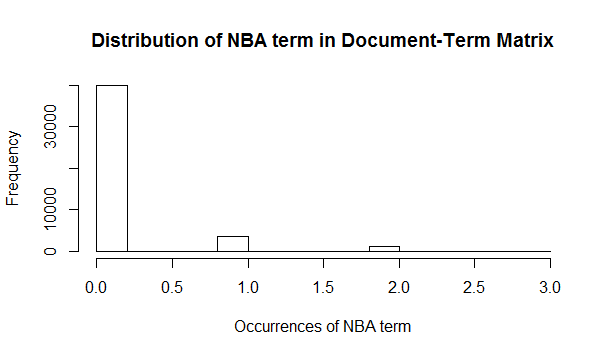
\includegraphics[width=\columnwidth]{nba.png}
	\caption{Non-Gaussian distribution of NBA in document-term matrix}
	\label{fig:1}
\end{figure}

To explore whether we could achieve higher accuracy with other classification techniques, we reduced the data set to 500 tweets per class for a total of 2500, using 70\% for training and 30\% for test. This reduction enabled our experiments to complete in a reasonable amount of time. For Naive-Bayes we noted a revised accuracy of 38\%. Random Forest achieved an accuracy of 27\% as per Table \ref{Tab:4} and SVM achieved an accuracy of 24\% as per Table \ref{Tab:5} .
\begin{table}[ht]
	\begin{center}
		\begin{tabular}{|c|c c c c c|}
			\hline
			\diagbox[width=8em]{actual}{predicted}& baseball & basketball & hockey & tennis& volleyball\\
			\hline
			baseball & 12&51&16&43&40\\
			basketball &2&52&12&27&33\\
			hockey & 14&52&11&47&46\\
			tennis &6&35&5&65&18\\
			volleyball& 7&54&22&20&60\\
			\hline
		\end{tabular}
	\end{center}
	\caption{Acutal vs predicted sports as classified by a Random Forest model trained on a reduced dataset}\label{Tab:4}
\end{table}
\begin{table}[ht]
	\begin{center}
		\begin{tabular}{|c|c c c c c|}
			\hline
			\diagbox[width=8em]{actual}{predicted}& baseball & basketball & hockey & tennis& volleyball\\
			\hline
			baseball &12&66&23&33&28\\
			basketball &5&56&13&24&28\\
			hockey &18&65 &12&37&38\\
			tennis &15&43&4&49&18\\
			volleyball&11&60&21&18&53\\
			\hline
		\end{tabular}
	\end{center}
	\caption{Actual vs predicted sports as classified by SVM with a radial kernel and trained on a reduced dataset}\label{Tab:5}
\end{table}

The SVM classification accuracy for various kernels is plotted in Figure 2.
\begin{figure}[!hbt]
	\centering
	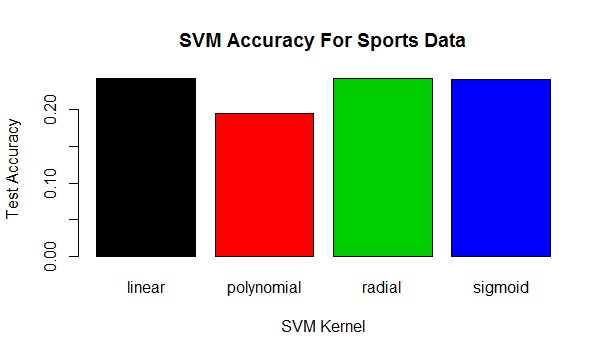
\includegraphics[width=\columnwidth]{compare.png}
	\caption{SVM Test Accuracy as achieved by various kernels on the reduced dataset}
	\label{fig:2}
\end{figure}

Clearly, our experiments show that after cleaning tweets of the hashtag labels for the sports under consideration, the best test accuracy attainable with conventional methods is 39\%. We now describe our LSTM model and demonstrate its superiority on this task.

\section{Predictive Modeling}
\subsection{Feature Engineering/extraction}
Each data point in the raw input data set is a tweet that consists of a list of words, which we convert to vector representation and use as the input features to our model. As we have seen previously, using term frequency as the features of each tweet has its limitations since it does not capture semantic information very well. Word2vec techniques, more specifically the Skip-Gram model is used here to convert a string of words to a vector representation of features Figure \ref{fig:3}.
\begin{figure}[!hbt]
	\centering
	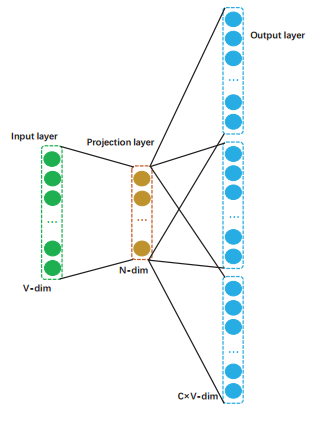
\includegraphics[width=0.8\columnwidth]{word2vec.png}
	\caption{ The skip-gram model architecture \cite{Li-lstm}.}
	\label{fig:3}
\end{figure}

The skip-gram model utilizes a shallow one-layer neural network to learn the representation of words such that the likelihood of obtaining surrounding words from a given word is maximized. In this project, we mapped each unique word into a 600-d low dimensional(comparing to one-hot encoding) vector space, i.e. the number of features used in our project is 600. We could convert the data to even higher dimensional feature spaces, but that would slow the training and is not necessary as the model is already performing very well.
\subsection{Model Design}
In Li et al \cite{Li-lstm}, they first start with a one-hot word representation, pass it through word2vec layers and form a distributed word representation. Then a convolutional neural network (CNN) is applied to each sentence in a tweet to extract local semantic information, and finally the output of the CNN is fed to Long Short-Term Memory (LSTM) layer. 

Due to time constraints, in this project our model architecture is different from theirs. We directly use an already trained word2vec model on Wikipedia Text8 corpus to encode each word in the input tweets, instead of training the word2vec representation ourselves. There is no sentence composition, that is we do not apply CNN on each sentence in a tweet. Instead, the memory cell in the LSTM layer is directly connected to each vector represented word in our model, and the final output is the predicted topic of that tweet, see Figure \ref{fig:4}. We do not use softmax layer for the classification.
\begin{figure}[!hbt]
	\centering
	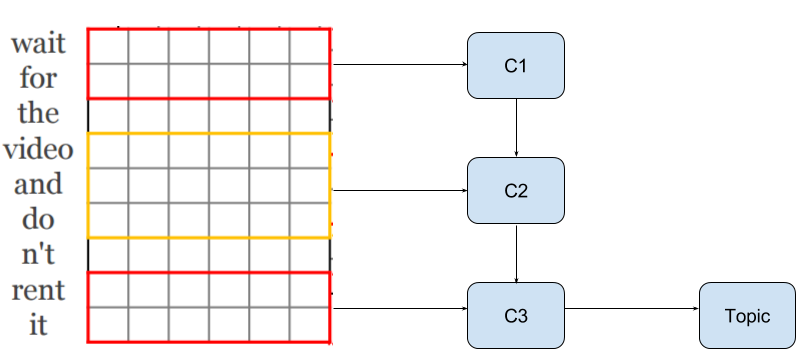
\includegraphics[width=\columnwidth]{cell.png}
	\caption{Each word in sentence connects to a LSTM cell}
	\label{fig:4}
\end{figure}

Each of the memory cells contains 4 major operations: 
\begin{itemize}
\item Forget gate: Provide a control over how much information comes through from previous cell.
\item Input node: Activation from input data at current time step.
\item Internal gate: Update and provide different candidate.
\item Ouput gate: Decide what to output and also what gets passed to next memory cell.
\end{itemize} 
\subsection{Build Model}
\subsubsection{Train}
Combine all sports tweets collected into one data set, with total 44,755 number of tweets. Train the model with a stratified 5-fold cross validation, each with 75\% training set and 25\% validation set. 

The number of hidden neurons is 300, the number of memory cells is 23 which is our sentence length (number of words), the dimension of each word is 600 as mentioned previously (so the total input data dimension is 23x600). We use a batch size of 50 and 20 epochs to train our model.\\ 
\subsubsection{Validation}
Predictions are made on the 25\% validation set from previous split, 5 times in total.\\
\subsubsection{Result}
The evaluation metric of the result on the validation set is \textit{harsh accuracy} which is the mean of the accuracy per class. 

Table \ref{Tab:6} shows the result of the first cross validation.
\begin{table}[ht]
		\scalebox{0.87}{\begin{tabular}{|c|ccccc|c|}
			\hline
			\diagbox[width=8em]{actual}{predicted}& baseball & basketball & hockey & tennis& volleyball&Accuracy\\
			\hline
			baseball &2335&35&28&64&27&0.9381\\
			basketball &53&2356&52&78&42&0.9128\\
			hockey &24&48&2289&56&16&0.9408\\
			tennis & 44&56&35&2342&32&0.9334\\
			volleyball&23&42&28&72&1012&0.8598\\
			\hline
		\end{tabular}}
	\caption{LSTM prediction result of 1st cross validation: confusion matrix and accuracy per class }\label{Tab:6}
\end{table}

Finally, we show the complete result of accuracy per class and harsh accuracy for each fold in the cross validation in Figure \ref{fig:5}:
\begin{figure}[!hbt]
	\centering
	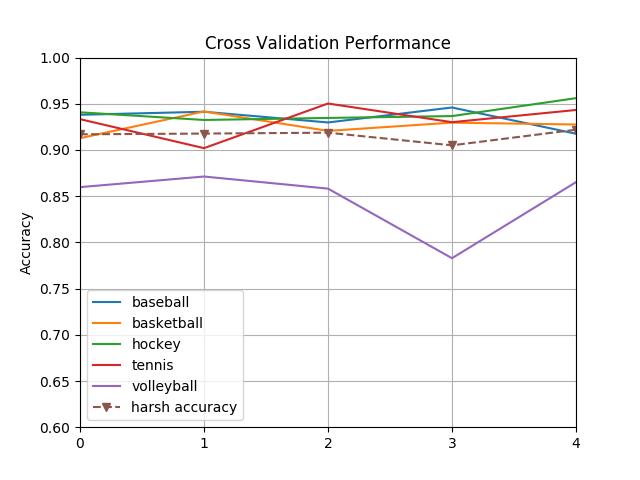
\includegraphics[width=\columnwidth]{cv.png}
	\caption{Accuracy per class and overall harsh accuracy for each validation set}
	\label{fig:5}
\end{figure}


We see that it achieves a remarkable result on this 5-class sports classification task, with high harsh accuracy and low variance. Although the model's prediction on \textit{volleyball} does not perform as well as the other topics, this is probably due to the relatively small size of the volleyball data set compared to the other collected sports.
\section{conclusion}
In this project, we developed a deep learning system to simulate the assignment of a sports topic hashtag to tweets that do not have one. We limited the scope of our work to classifying a tweet as one of five popular sports. The deep learning architecture chosen was an LSTM neural network fed with input consisting of the words of a tweet represented as vectors. The output of the LSTM was used directly for the class probability. The system achieved a test accuracy of 92\%.

To compare our results to more conventional techniques, we performed a series of benchmark experiments on a data set that was reduced in size. These experiments used the TF-IDF method to obtain a document-term matrix before applying a classifier. Naive-Bayes, Random Forest, and SVM achieved test accuracy scores of 38\%, 27\%, and 24\% respectively. Clearly, LSTM, with word2vec representations as input, greatly outperforms them all.

For future work, the model could possibly be brought more in line with that of Li et al \cite{Li-lstm} by using a CNN for the sentences of a tweet which feeds an LSTM with its representations. With more computing resources, the number of different sports used as class labels could also be increased.

\begin{thebibliography}{5}

	%Each item starts with a \bibitem{reference} command and the details thereafter.
	\bibitem{Li-lstm} % Transaction paper
	J. Li, H. Xu, X. He, J. Deng and X. Sun. Tweet Modeling with LSTM Recurrent Neural
	Networks for Hashtag Recommendation {\em International Joint Conference on Neural Networks (IJCNN)}, 2016

	\bibitem{word2vec} % Conference paper
	T. Mikolov, I. Sutskever, K. Chen, G. Corrado, J. Dean. 2013. Distributed Representations of Words and Phrases and their Compositionality. {\em In Proceedings of NIPS}, 2013.

	\bibitem{classw2v}
	R. Collobert, J. Weston, L. Bottou, M. Karlen, K.Kavukcuglu, P. Kuksa. 2011. Natural Language Processing (Almost) from Scratch. Journal of Machine Learning Research 12:2493–2537
\end{thebibliography}

% Your document ends here!
\end{document}